\documentclass[10pt]{article}
\usepackage[T1]{fontenc}

% Document Details
\newcommand{\CLASS}{AMATH 585}
\newcommand{\assigmentnum}{Assignment 5}

\usepackage[margin = 1.15in, top = 1.25in, bottom = 1.in]{geometry}

\usepackage{titling}
\setlength{\droptitle}{-6em}   % This is your set screw
\date{}
\renewcommand{\maketitle}{
	\clearpage
	\begingroup  
	\centering
	\LARGE \sffamily\textbf{\CLASS} \Large \assigmentnum\\[.8em]
	\large Tyler Chen\\[1em]
	\endgroup
	\thispagestyle{empty}
}
 % Title Styling
\usepackage{tocloft}
\renewcommand{\cfttoctitlefont}{\Large\sffamily\bfseries}
\renewcommand{\cftsecfont}{\normalfont\sffamily\bfseries}
\renewcommand{\cftsubsecfont}{\normalfont\sffamily}
\renewcommand{\cftsubsubsecfont}{\normalfont\sffamily}

\makeatletter
\let\oldl@section\l@section
\def\l@section#1#2{\oldl@section{#1}{\sffamily\bfseries#2}}

\let\oldl@subsection\l@subsection
\def\l@subsection#1#2{\oldl@subsection{#1}{\sffamily#2}}

\let\oldl@subsubsection\l@subsubsection
\def\l@subsubsection#1#2{\oldl@subsubsection{#1}{\sffamily#2}}
 % General Styling


\usepackage{enumitem}

% Figures
\usepackage{subcaption}

% TikZ and Graphics
\usepackage{tikz, pgfplots}
\pgfplotsset{compat=1.12}
\usetikzlibrary{patterns,arrows}
\usepgfplotslibrary{fillbetween}

\usepackage{pdfpages}
\usepackage{adjustbox}

\usepackage{lscape}
\usepackage{titling}
\usepackage[]{hyperref}


% Header Styling
\usepackage{fancyhdr}
\pagestyle{fancy}
\lhead{\sffamily \CLASS}
\rhead{\sffamily Chen \textbf{\thepage}}
\cfoot{}

% Paragraph Styling
\setlength{\columnsep}{1cm}
\setlength{\parindent}{0pt}
\setlength{\parskip}{5pt}
\renewcommand{\baselinestretch}{1}

% TOC Styling
\usepackage{tocloft}
\iffalse
\renewcommand{\cftsecleader}{\cftdotfill{\cftdotsep}}

\renewcommand\cftchapafterpnum{\vskip6pt}
\renewcommand\cftsecafterpnum{\vskip10pt}
\renewcommand\cftsubsecafterpnum{\vskip6pt}

% Adjust sectional unit title fonts in ToC
\renewcommand{\cftchapfont}{\sffamily}
\renewcommand{\cftsecfont}{\bfseries\sffamily}
\renewcommand{\cftsecnumwidth}{2em}
\renewcommand{\cftsubsecfont}{\sffamily}
\renewcommand{\cfttoctitlefont}{\hfill\bfseries\sffamily\MakeUppercase}
\renewcommand{\cftaftertoctitle}{\hfill}

\renewcommand{\cftchappagefont}{\sffamily}
\renewcommand{\cftsecpagefont}{\bfseries\sffamily}
\renewcommand{\cftsubsecpagefont}{\sffamily}
\fi
 % General Styling
% Code Display Setup
\usepackage{listings,lstautogobble}
\usepackage{lipsum}
\usepackage{courier}
\usepackage{catchfilebetweentags}

\lstset{
	basicstyle=\small\ttfamily,
	breaklines=true, 
	frame = single,
	rangeprefix=,
	rangesuffix=,
	includerangemarker=false,
	autogobble = true
}


\usepackage{algorithmicx}
\usepackage{algpseudocode}

\newcommand{\To}{\textbf{to}~}
\newcommand{\DownTo}{\textbf{downto}~}
\renewcommand{\algorithmicdo}{\hspace{-.2em}\textbf{:}}
 % Code Display Setup
% AMS MATH Styling
\usepackage{amsmath, amssymb}
\newcommand{\qed}{\hfill\(\square\)}

%\newtheorem*{lemma}{Lemma} 
%\newtheorem*{theorem}{Theorem}
%\newtheorem*{definition}{Definition}
%\newtheorem*{prop}{Proposition}
%\renewenvironment{proof}{{\bfseries Proof.}}{}


% mathcal
\newcommand{\cA}{\ensuremath{\mathcal{A}}}
\newcommand{\cB}{\ensuremath{\mathcal{B}}}
\newcommand{\cC}{\ensuremath{\mathcal{C}}}
\newcommand{\cD}{\ensuremath{\mathcal{D}}}
\newcommand{\cE}{\ensuremath{\mathcal{E}}}
\newcommand{\cF}{\ensuremath{\mathcal{F}}}
\newcommand{\cG}{\ensuremath{\mathcal{G}}}
\newcommand{\cH}{\ensuremath{\mathcal{H}}}
\newcommand{\cI}{\ensuremath{\mathcal{I}}}
\newcommand{\cJ}{\ensuremath{\mathcal{J}}}
\newcommand{\cK}{\ensuremath{\mathcal{K}}}
\newcommand{\cL}{\ensuremath{\mathcal{L}}}
\newcommand{\cM}{\ensuremath{\mathcal{M}}}
\newcommand{\cN}{\ensuremath{\mathcal{N}}}
\newcommand{\cO}{\ensuremath{\mathcal{O}}}
\newcommand{\cP}{\ensuremath{\mathcal{P}}}
\newcommand{\cQ}{\ensuremath{\mathcal{Q}}}
\newcommand{\cR}{\ensuremath{\mathcal{R}}}
\newcommand{\cS}{\ensuremath{\mathcal{S}}}
\newcommand{\cT}{\ensuremath{\mathcal{T}}}
\newcommand{\cU}{\ensuremath{\mathcal{U}}}
\newcommand{\cV}{\ensuremath{\mathcal{V}}}
\newcommand{\cW}{\ensuremath{\mathcal{W}}}
\newcommand{\cX}{\ensuremath{\mathcal{X}}}
\newcommand{\cY}{\ensuremath{\mathcal{Y}}}
\newcommand{\cZ}{\ensuremath{\mathcal{Z}}}

% mathbb
\usepackage{bbm}
\newcommand{\bOne}{\ensuremath{\mathbbm{1}}}

\newcommand{\bA}{\ensuremath{\mathbb{A}}}
\newcommand{\bB}{\ensuremath{\mathbb{B}}}
\newcommand{\bC}{\ensuremath{\mathbb{C}}}
\newcommand{\bD}{\ensuremath{\mathbb{D}}}
\newcommand{\bE}{\ensuremath{\mathbb{E}}}
\newcommand{\bF}{\ensuremath{\mathbb{F}}}
\newcommand{\bG}{\ensuremath{\mathbb{G}}}
\newcommand{\bH}{\ensuremath{\mathbb{H}}}
\newcommand{\bI}{\ensuremath{\mathbb{I}}}
\newcommand{\bJ}{\ensuremath{\mathbb{J}}}
\newcommand{\bK}{\ensuremath{\mathbb{K}}}
\newcommand{\bL}{\ensuremath{\mathbb{L}}}
\newcommand{\bM}{\ensuremath{\mathbb{M}}}
\newcommand{\bN}{\ensuremath{\mathbb{N}}}
\newcommand{\bO}{\ensuremath{\mathbb{O}}}
\newcommand{\bP}{\ensuremath{\mathbb{P}}}
\newcommand{\bQ}{\ensuremath{\mathbb{Q}}}
\newcommand{\bR}{\ensuremath{\mathbb{R}}}
\newcommand{\bS}{\ensuremath{\mathbb{S}}}
\newcommand{\bT}{\ensuremath{\mathbb{T}}}
\newcommand{\bU}{\ensuremath{\mathbb{U}}}
\newcommand{\bV}{\ensuremath{\mathbb{V}}}
\newcommand{\bW}{\ensuremath{\mathbb{W}}}
\newcommand{\bX}{\ensuremath{\mathbb{X}}}
\newcommand{\bY}{\ensuremath{\mathbb{Y}}}
\newcommand{\bZ}{\ensuremath{\mathbb{Z}}}

% alternative mathbb
\newcommand{\NN}{\ensuremath{\mathbb{N}}}
\newcommand{\RR}{\ensuremath{\mathbb{R}}}
\newcommand{\CC}{\ensuremath{\mathbb{C}}}
\newcommand{\ZZ}{\ensuremath{\mathbb{Z}}}
\newcommand{\EE}{\ensuremath{\mathbb{E}}}
\newcommand{\PP}{\ensuremath{\mathbb{P}}}
\newcommand{\VV}{\ensuremath{\mathbb{V}}}
\newcommand{\cov}{\ensuremath{\text{Co}\VV}}
% Math Commands

\newcommand{\st}{~\big|~}
\newcommand{\stt}{\text{ st. }}
\newcommand{\ift}{\text{ if }}
\newcommand{\thent}{\text{ then }}
\newcommand{\owt}{\text{ otherwise }}

\newcommand{\norm}[1]{\left\lVert#1\right\rVert}
\newcommand{\snorm}[1]{\lVert#1\rVert}
\newcommand{\ip}[1]{\ensuremath{\left\langle #1 \right\rangle}}
\newcommand{\pp}[3][]{\frac{\partial^{#1}#2}{\partial #3^{#1}}}
\newcommand{\dd}[3][]{\frac{\d^{#1}#2}{\d #3^{#1}}}
\renewcommand{\d}{\ensuremath{\mathrm{d}}}

\newcommand{\indep}{\rotatebox[origin=c]{90}{$\models$}}




 % Math shortcuts
% Problem
\usepackage{floatrow}

\newenvironment{problem}[1][]
{\pagebreak
\noindent\rule{\textwidth}{1pt}\vspace{0.25em}
{\sffamily \textbf{#1}}
\par
}
{\par\vspace{-0.5em}\noindent\rule{\textwidth}{1pt}}

\newenvironment{solution}[1][]
{{\sffamily \textbf{#1}}
\par
}
{}

 % Problem Environment

\newcommand{\note}[1]{\textcolor{red}{\textbf{Note:} #1}}

\hypersetup{
   colorlinks=true,       % false: boxed links; true: colored links
   linkcolor=violet,          % color of internal links (change box color with linkbordercolor)
   citecolor=green,        % color of links to bibliography
   filecolor=magenta,      % color of file links
   urlcolor=cyan           % color of external links
}


\begin{document}
\maketitle



\begin{problem}[Problem 1]
Write a code to solve Poisson's equation on the unit square with Dirichlet
boundary conditions:
\[
u_{xx} + u_{yy} = f(x,y) ,~~~0 < x,y < 1 
\]
\[
u(x,0) = u(x,1) = u(0,y) = u(1,y) = 1.
\]
Take \( f(x,y) = x^2 + y^2 \), and demonstrate numerically that your code 
achieves second order accuracy.  [Note:  If you do not know an analytic
solution to a problem, one way to check the code is to solve the problem
on a fine grid and pretend that the result is the exact solution, then
solve on coarser grids and compare your answers to the fine grid solution.
However, you must be sure to compare solution values corresponding to
the same points in the domain.]
\end{problem}

\begin{solution}[Solution]

We implement our five point stencil for solving the Poisson equation in Python.
\lstinputlisting[linerange=\#<startTeX>-\#<endTeX>, gobble = 4]{hw5_1.py}

This gives solutions shown in Figure~\ref{5ptsol}.
\begin{figure}[H]\centering
    \foreach \m in {3,7,15,31}{%,63,127,255}{
        \begin{subfigure}{.23\textwidth}
            \includegraphics[width=\textwidth]{img/1/\m.pdf}
            \caption{\(m = \m\)}
        \end{subfigure}
    }
\caption{Solutions using 5 point Laplacian with \( m \) interior points in each direction}
\label{5ptsol}
\end{figure}

We now analyze the results by comparing the results on a coarse mesh to those on a finer mesh. By plotting the error vs the mesh width on a log-log plot, the slope will give the order of convergence. This is done in Figure~\ref{5pt}. As expected the convergence is order \( h^2 \).

    \begin{figure}[H]\centering
    \begin{subfigure}{.48\textwidth}
        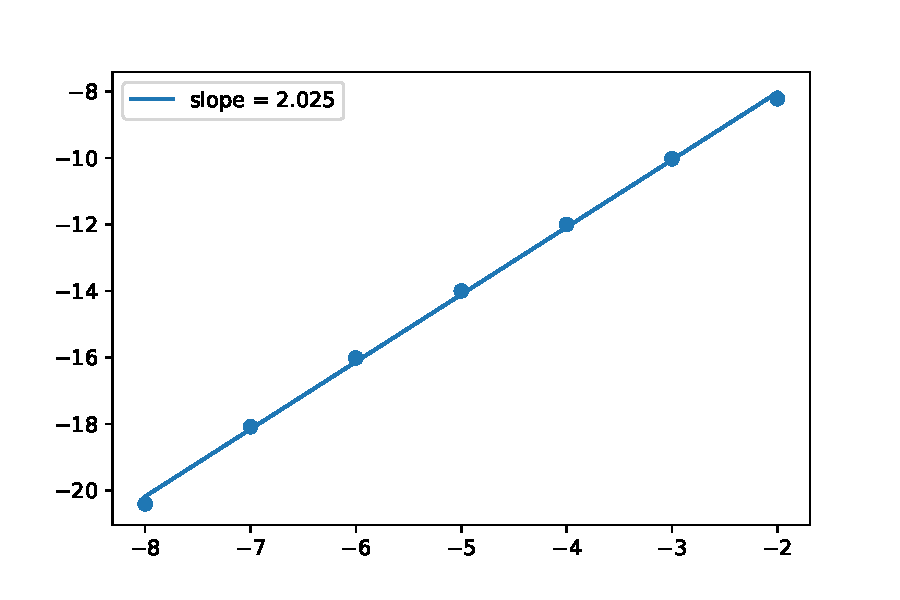
\includegraphics[width=\textwidth]{img/1/error_inf.pdf}
        \caption{\(\log h\) vs. \( \log\norm{\text{error}}_\infty \)}
    \end{subfigure}
    \begin{subfigure}{.48\textwidth}
        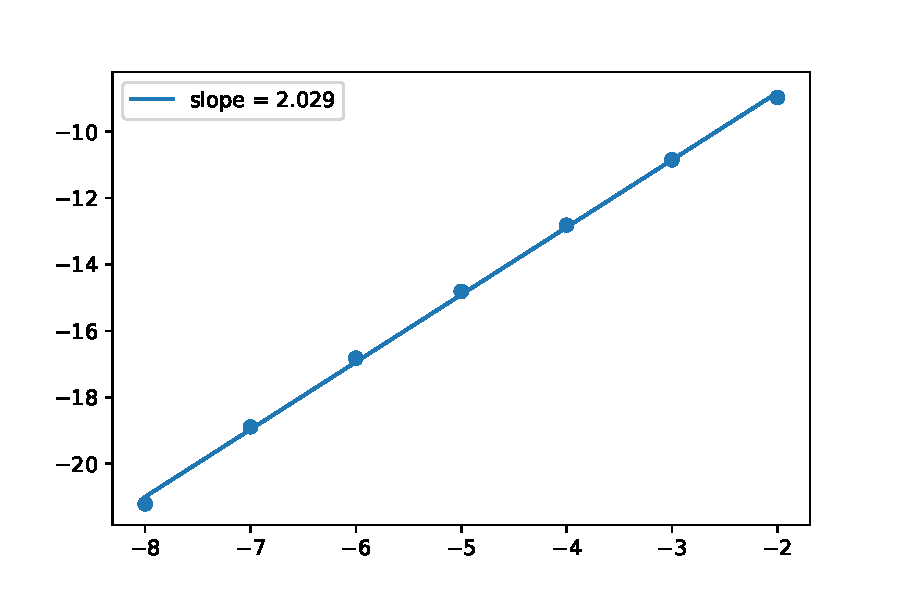
\includegraphics[width=\textwidth]{img/1/error_2.pdf}
        \caption{\(\log h\) vs. \( \log\norm{\text{error}}_{L2} \)}
    \end{subfigure}
\caption{Error vs fine mesh for 5-point Laplacian}
\label{5pt}
\end{figure}


\end{solution}

\begin{problem}[Problem 2]
Now use the 9-point formula with the correction term described in Sec. 3.5 to solve
the same problem as in the previous exercise.
Again take \( f(x,y) = x^2 + y^2 \), and numerically test the order of accuracy of your code
by solving on a fine grid, pretending that is the exact solution, and comparing 
coarser grid approximations to the corresponding values of the fine grid solution.
Show what order of accuracy you achieve and try to explain why.
\end{problem}

\begin{solution}[Solution]

We have 9-point formula given as,
\begin{align*}
    \nabla_9^2 u_{ij} = \dfrac{1}{6h^2} \left[ 4 u_{i-1,j} + 4u_{i+1,j} + 4u_{i,j-1}+4u_{i,j+1}+u_{i-1,j-1}+u_{i-1,j+1}+u_{i+1,j-1}+u_{i+1,j+1}-20u_{ij} \right]
\end{align*}

Given that \( u \) is sufficiently smooth we have,
\begin{align*}
    \dfrac{1}{12} h^2 (u_{xxxx}+2u_{xxyy}+u_{yyyy}) + \mathcal{O}(h^4)
\end{align*}

We note that,
\begin{align*}
    u_{xxxx}+2u_{xxyy}+u_{yyyy} = \nabla^2(\nabla^2u) = \nabla^2 f
\end{align*}

Therefore we have fourth order accurate finite difference method given by,
\begin{align*}
    \nabla_9^2 u_{ij} = f(x_i,y_j) + \dfrac{h^2}{12} \nabla^2 f(x_i,y_j)
\end{align*}

In this problem we have,
\begin{align*}
    \nabla^2 f = f_{xx} + f_{yy} = 2+2 =4
\end{align*}

The matrix equation corresponding to this finite difference method is of the form,
\begin{align*}
    Au = f
\end{align*}
where
\begin{align*}
    A = \left[\begin{array}{cccc}
    T & S\\
        S &\ddots & \ddots \\
    & \ddots & \ddots & S\\
    & & S & T
    \end{array}\right]
    , &&
    T = \left[\begin{array}{cccc}
    -20 & 4 \\
        4 & \ddots & \ddots \\
        & \ddots & \ddots & 4\\
    & & 4 & -20\end{array}\right]
    ,&& S = \left[\begin{array}{cccc}
    4 & 1 \\
        1 & \ddots & \ddots \\
        & \ddots & \ddots & 1\\
    & & 1 & 4\end{array}\right]
\end{align*}
and, given \( f = x^2+y^2 \) so that \( \nabla^2 f = 4 \),
\begin{align*}
    f_{ij} = x_i^2+x_j^2 - \partial u_{ij}/h^2 + 4, &&
    \partial u_{ij} = 6|\{i,j\}\cap\{1,m\}| - \max(0,|\{i,j\} \cap \{1,m\}|-1)
\end{align*}
\iffalse
where,
\begin{align*}
    \partial u_{ij} = \begin{cases}
        11 & |\{i,j\}\cap\{1,m\}| = 2 \\
        6 & |\{i,j\} \cap\{1,m\}| = 1 \\
        0 & |\{i,j\} \cap \{1,m\}| = 0
    \end{cases}
\end{align*}
    \partial u = \left[\begin{array}{ccccc}
        2 & 1 & \cdots & 1 & 2 \\
        1 & & & & 1 \\
        \vdots & & & & \vdots \\
        1 & & & & 1 \\
        2 & 1 & \cdots & 1 & 2 
    \end{array}\right]
\fi

We implement our nine point stencil for solving the Poisson equation in Python.
\lstinputlisting[linerange=\#<startTeX>-\#<endTeX>, gobble = 4]{hw5_2.py}

This gives solutions shown in Figure~\ref{9ptsol}.
\begin{figure}[H]\centering
    \foreach \m in {3,7,15,31}{%,63,127,255,511}{
        \begin{subfigure}{.23\textwidth}
            \includegraphics[width=\textwidth]{img/2/\m.pdf}
            \caption{\( m = \m \) }
        \end{subfigure}
    }
\caption{Solutions using 9 point Laplacian with \( m \) interior points in each direction}
\label{9ptsol}
\end{figure}

As before the errors are plotted on a log-log plot. We use a grid as fine as \( 1023 \times 1023 \) interior points which corresponds to solving a system with over a million equations!
\begin{figure}[H]\centering
    \begin{subfigure}{.48\textwidth}
        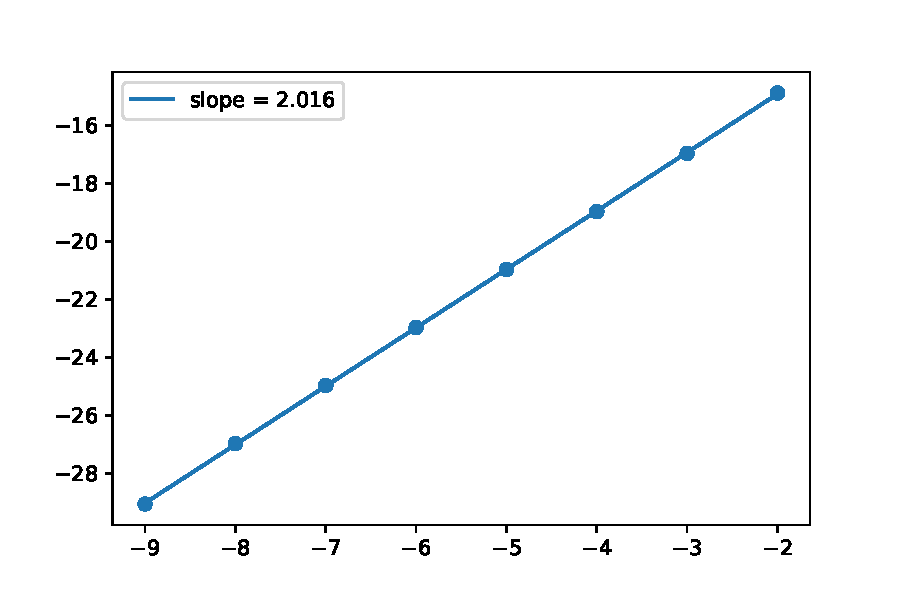
\includegraphics[width=\textwidth]{img/2/error_inf.pdf}
        \caption{\(\log h\) vs. \( \log\norm{\text{error}}_\infty \)}
    \end{subfigure}
    \begin{subfigure}{.48\textwidth}
        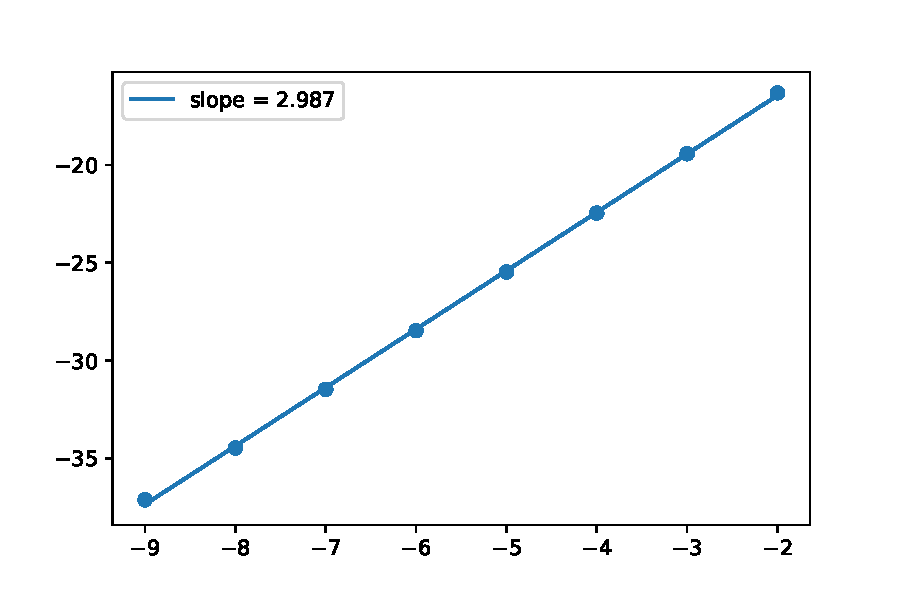
\includegraphics[width=\textwidth]{img/2/error_2.pdf}
        \caption{\(\log h\) vs. \( \log\norm{\text{error}}_{L2} \)}
    \end{subfigure}
\caption{Error vs fine mesh for 9-point Laplacian}
\label{9pt}
\end{figure}


The condition for using this error correction to get order \( h^4 \) convergence was the smoothness of \( u \). In particular, we require \( u_{xxxx},u_{xxyy},u_{yyyy} \) to all exist. 

However, our boundary conditions correspond to a level curve of \( u \) in the shape of a square. In the corners we have \( u_x = u_y = 0 \) so that \( \nabla^2 u = u_{xx}+u_{yy} = 0 \). However, \( \nabla^2 u = f(x,y) = x^2+y^2 \) is nonzero at \( (0,1), (1,0), \) and \( (1,1) \). This means there is some discontinuity in \( u_{xx}+u_{yy} \) as we approach these corners. 

As seen in our numerical results, this is enough to change the error term in our analysis and prevent \( h^4 \) convergence.



\end{solution}

\begin{problem}[Problem 3] 
We have discussed using finite element methods to solve elliptic PDE's such as 
\[
\bigtriangleup u = f~~\mbox{ in } \Omega ,~~~u = 0~~\mbox{ on } \partial \Omega ,
\]
with {\em homogeneous} Dirichlet boundary conditions.  How could you modify the procedure
to solve the {\em inhomogeneous} Dirichlet problem:
\[
\bigtriangleup u = f~~\mbox{ in } \Omega ,~~~u = g~~\mbox{ on } \partial \Omega ,
\]
where \( g \) is some given function?  Derive the equations that you would need to
solve to compute, say, a continuous piecewise bilinear approximation for this problem
when \( \Omega \) is the unit square \( (0,1) \times (0,1) \).
\end{problem}

\begin{solution}[Solution]

We seek a solution to \( \mathcal{L} u = f \) in \( \Omega = (0,1)\times(0,1) \) given some boundary condition \( u = g \) on \( \partial \Omega \).

With homogeneous Dirichlet boundary conditions of zero we have,
\begin{align*}
    S = \{ \varphi : \varphi \text{ is a continuous bilinear function on given grid with } \varphi(\omega) = 0, \forall \omega\in\partial\Omega \}
\end{align*}

Define an inner product \( \langle \cdot, \cdot\rangle : S\times S\to\RR_+ \) by,
\begin{align*}
    \langle f, g\rangle = \iint_\Omega f\cdot g~ dA
\end{align*}

Note that when we write \( \langle \mathcal{L} \hat{u},\hat{v} \rangle \) we mean the value of the integral after applying Green's theorem as \( \mathcal{L} \hat{u} \) may not be well defined if \( \hat{u} \) is not sufficiently smooth. In particular, with \( \mathcal{L} u = \nabla^2 u = u_xx + u_yy \) we have,
\begin{align*}
    \langle \mathcal{L} \hat{u},\hat{v} \rangle  = 
    \iint_\Omega (\hat{u}_{xx} + \hat{u}_{yy}) \hat{v} dA
    = - \iint_\Omega (\hat{u}_x\hat{v}_x+\hat{u}_y\hat{v}_y)dA + \int_{\partial\Omega} \hat{u}_{n}\hat{v} d\gamma
\end{align*}
where \( \hat{u}_n \) is the derivative of \( \hat{u} \) in the outward normal direction along the boundary. Note further that if \( \hat{v} = 0 \) (as is the case for entries of \( A \) and \( F \) below) on \( \partial \Omega \) that the second term is zero.




We extend the current set of basis functions for \( S \) to span the set of all piecewise bilinear functions on the given grid, denoted \( S' \).

Let \( \{x_0,x_1, \ldots, x_{n_x},x_{n_x+1}\} \times\{y_0,y_1, \ldots, y_{n_y},y_{n_y+1}\} \) define the mesh for \( S \).
A basis \( B \) for \( S \) is \( B =\{ \varphi_{k} \}_{k=1}^{n_xn_y} \), where \( \varphi_{i+(j-1)n_x}(x,y) \) is centered at \( (x_i,y_j) \) and is defined as,
\begin{align*}
    \varphi_{i + (j-1)n_x}(x,y) = 
    \begin{cases}
        (x-x_{i-1})(y-y_{j-1})/(x_i-x_{i-1})(y_j-y_{j-1}) & \text{in }[x_{i-1},x_i]\times [y_{j-1},y_j] \\
        (x-x_{i+1})(y-y_{j-1})/(x_i-x_{i+1})(y_j-y_{j-1}) & \text{in }[x_{i},x_{i+1}]\times [y_{j-1},y_j] \\
        (x-x_{i-1})(y-y_{j+1})/(x_i-x_{i-1})(y_j-y_{j+1}) & \text{in }[x_{i-1},x_i]\times [y_{j},y_{j+1}] \\
        (x-x_{i+1})(y-y_{j+1})/(x_i-x_{i+1})(y_j-y_{j+1}) & \text{in }[x_{i},x_{i+1}]\times [y_{j},y_{j+1}] \\
        0 & \text{otherwise}
    \end{cases}
\end{align*}

We now extend \( B \) to a basis \( B' \) for \( S' \). Indeed, take the above definition, except, since \( x_{-1}, x_{n_x+2}, y_{-1}, y_{n_y+2} \) are not defined, ignore the definition in regions which would be outside \( [0,1]\times[0,1] \). Let all such functions be called \( B' \).


Clearly \( |B'| = (n_x+2)(n_y+2) \) which is the dimension of \( S' \) as functions in \( S' \) have this many free parameters. Moreover, they elements of \( B' \) are linearly independent since they do not overlap at the centers.
This proves \( B' \) is a basis for \( S' \).

Keep the numbering for the basis for \( S \) and append the new vectors with some new ordering. For convenience define \( M = n_xn_y \) and \( N = (n_x+2)(n_y+2) \). That is, \( M = |B| \) and \( N = |B'| \).

With the new basis our approximate solution \( \hat{u} \) to the differential equation \( \mathcal{L}u=f \) is of the form,
\begin{align*}
    \hat{u} = \sum_{k=1}^{N} c_k \varphi_k
\end{align*}
Given boundary condition \( u=g \) on the boundary we have \( c_k = g(x_i,y_j) \) for \( k=M+1,\ldots N\), where \( \varphi_k \) is centered at \( (x_i,y_j) \).

This leaves \( M \) unknown coefficients. Thus, for any \( k=1,...,M \), write,
\begin{align*}
    \langle f, \varphi_k \rangle = \langle \mathcal{L} \hat{u} , \varphi_k \rangle 
    = \sum_{n=1}^{N} c_n\langle \mathcal{L}\varphi_n,\varphi_k \rangle
    = \sum_{n=1}^{M} c_n\langle \mathcal{L}\varphi_n,\varphi_k \rangle
    + \sum_{n=M+1}^{N} c_n\langle \mathcal{L}\varphi_n,\varphi_k \rangle
\end{align*}

Since we know the value of \( c_n \) for all \( n\in\{M+1, \ldots, N\} \) we can subtract the second sum from \( \langle f,\varphi_k \rangle \). This means the matrix \( A \) will be the same as previously. However, the right hand side \( F \) will be changed.

Specifically, we are solving \( AC = F \) where, for \( k,n\in\{1,2,\ldots, n_xn_y\} \),
\begin{align*}
    A_{k,n} = \langle \mathcal{L} \varphi_n, \varphi_k \rangle, && C_n = c_n, &&
    F_{k} = \langle f, \varphi_k \rangle - \sum_{n=M+1}^{N} c_n \langle \mathcal{L} \varphi_n, \varphi_k\rangle
\end{align*}

We make a few remarks. First, \( \langle \varphi_n,\varphi_m \rangle = 0 \) if \( \varphi_n \) and \( \varphi_m \) are not centered in adjacent grid points (diagonals included). This means the sums above can be simplified quite a bit by not evaluating needless things. Moreover, \( \langle \mathcal{L} \varphi_n, \varphi_k \rangle \) may have a nice closed form expression depending on \( \mathcal{L} \). In particular, if \( \mathcal{L} \) does not depend on \( x \) or \( y \), then only the relative positions of the centers of \( \varphi_n \) and \( \varphi_k \) are important.


\end{solution}

\begin{problem}[Problem 4]
The key to efficiency in the \verb+chebfun+ package, which you used in a previous homework
exercise, is the ability to rapidly translate between the values of a function at the
Chebyshev points, \( \cos ( \pi j/n ) \), \( j=0, \ldots , n \), and the coefficients \( a_0 , \ldots , a_n \),
in a Chebyshev expansion of the function's \( n \)th-degree polynomial interpolant:
\( p(x) = \sum_{j=0}^n a_j T_j (x) \), where \( T_j (x) = \cos ( j \arccos (x) ) \) is the \( j \)th
degree Chebyshev polynomial.  Knowing the coefficients \( a_0 , \ldots , a_n \), one can evaluate
\( p \) at the Chebyshev points by evaluating the sums
\begin{equation}
p ( \cos ( k \pi / n ) ) = \sum_{j=0}^n a_j \cos ( j k \pi / n ) ,~~~k=0, \ldots , n.
\label{Cheby}
\end{equation}
These sums are much like the real part of the sums in the FFT,
\[
F_k = \sum_{j=0}^{n-1} e^{2 \pi i j k / n} f_j ,~~~k=0, \ldots , n-1 ,
\]
but the argument of the cosine differs by a factor of \( 2 \) from the values that would make
them equal.  Explain how the FFT or a closely related procedure could be used to evaluate
the sums in (\ref{Cheby}).  To go in the other direction, and efficiently determine the coefficients
\( a_0 , \ldots , a_n \) from the function values \( f( \cos ( k \pi / n ) ) \), what method would you use?
\end{problem}

\begin{solution}[Solution]

First observe that for any integer \( k \) and \( n \) that,
\begin{align*}
    \cos \left( \dfrac{\pi(n-j)k}{n} \right) = \cos(\pi k)\cos \left( -\dfrac{\pi j k}{n} \right) = \cos(\pi k) \cos \left( \dfrac{\pi j k}{n} \right) = \cos \left( \dfrac{\pi(n+j)k}{n} \right)
    \\
    \sin \left( \dfrac{\pi(n-j)k}{n} \right) = \cos(\pi k)\sin \left( -\dfrac{\pi j k}{n} \right) = -\cos(\pi k) \sin \left( \dfrac{\pi j k}{n} \right) = -\sin \left( \dfrac{\pi(n+j)k}{n} \right)
\end{align*}

With this in mind, for \( j=1,2,\ldots, n \) define,
\begin{align*}
    a_{n+j} = a_{n-j}
\end{align*}

Then for any integer \( k=1,2,\ldots, n \) the DFT gives,
\begin{align*}
    A_k = \sum_{j=0}^{2n-1} a_j e^{\pi i j k / n} =  \sum_{j=0}^{2n-1}a_j \cos \left( \dfrac{\pi j k}{n} \right) + i a_j \sin \left( \dfrac{\pi j k}{n} \right)
\end{align*}

Therefore,
\begin{align*}
    a_0 + a_n e^{ik\pi} + A_k &= a_{2n} + a_n e^{\pi n k / n} + \sum_{j=0}^{n}a_je^{\pi i j k /n} + \sum_{j=n+1}^{2n-1}a_j e^{\pi i j k/n} 
    = \sum_{j=0}^{n} a_j e^{ \pi i j k / n} + \sum_{j=n}^{2n}a_j e^{\pi i j k /n}
\end{align*}

By the relationships between cosine and sine shown above the imaginary parts of these sums cancel, and the real parts are the same. That is, 
\begin{align*}
    a_0 + a_n e^{ik\pi} + A_k = 2\operatorname{Re} \left[ \sum_{j=0}^{n}a_j e^{\pi i j k/n} \right] = 2\sum_{j=0}^{n}a_j \cos \left( \dfrac{\pi j k}{n} \right)
\end{align*}

Therefore, 
\begin{align*}
    p(\cos(k \pi /n )) = \sum_{j=0}^{n} a_j \cos \left( \dfrac{\pi j k}{n} \right) = \dfrac{a_0 + (-1)^k a_n + A_k}{2}
\end{align*}

We can use the DFT to compute \( A_k \) in \( n\log n \) time so we can compute all of the \( p(\cos(k\pi/n)) \) in \( n\log n \) time. This is better than the \( n^2 \) time it would take to compute each of the \( n \) sums of \( n \) terms directly. 


Given \( p(\cos( k \pi / n)) \) for \( k=0,\ldots, n\) and assumign we know \( a_0 \) and \( a_n \) we can compute \( A_k \) for \( k=0,\ldots,n \).
We then would apply a similar process to above, but with the inverse DFT.

\end{solution}
\end{document}
